\section{Introduction}





%--------------------------------------------------
\slide{Unstable nuclei and the limits of stability} 

% -------------------------------------------------------------------------------------
\begin{figure}{\par \resizebox*{0.6\textwidth}{!}
{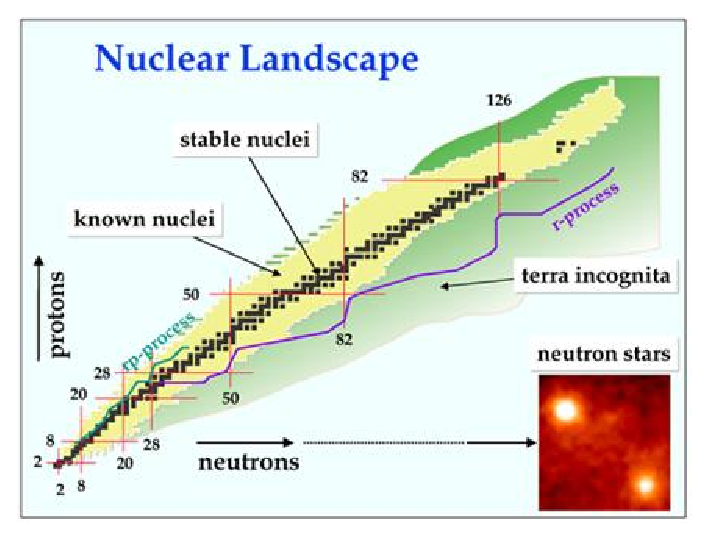
\includegraphics{figs/landscape.eps}} \par}
\end{figure}

Note that:
 \bi 
 \item Not all unstable nuclei are weakly-bound. 
 \item There are weakly-bound nuclei which are not unstable (eg.~deuteron).
 \ei

\end{frame}



% --------------------------------------------------------------------------------------
\slide{Light exotic nuclei: halo nuclei and Borromean systems}

\begin{figure}{\par \resizebox*{0.75\textwidth}{!}
{\includegraphics[angle=-90]{figs/segre.ps}} \par}
\end{figure}

\end{frame}

% --------------------------------------------------------------------------------------
\slide{Light exotic nuclei: halo nuclei and Borromean systems}

\begin{itemize}
\setlength{\itemsep}{11pt}
\gitem{Radioactive nuclei:} they typically decay by $\beta$ emission. \\
{\bf E.g.:}~\nuc{6}{He} $\xrightarrow{\beta ^{-}}$ \nuc{6}{Li} ~~~ ($\tau_{1/2}\simeq $807 ms)

\gitem{Weakly bound}: typical separation energies are around 1 MeV or less.

\gitem{Spatially extended}

\gitem{Halo structure:} one or two weakly bound nucleons (typically neutrons) with a large 
probability of presence beyond the range of the potential.

\gitem{Borromean nuclei:} Three-body systems with no bound binary sub-systems. 

\begin{columns}
\column{0.5\linewidth}
\begin{figure}{\par \resizebox*{0.45\textwidth}{!}
{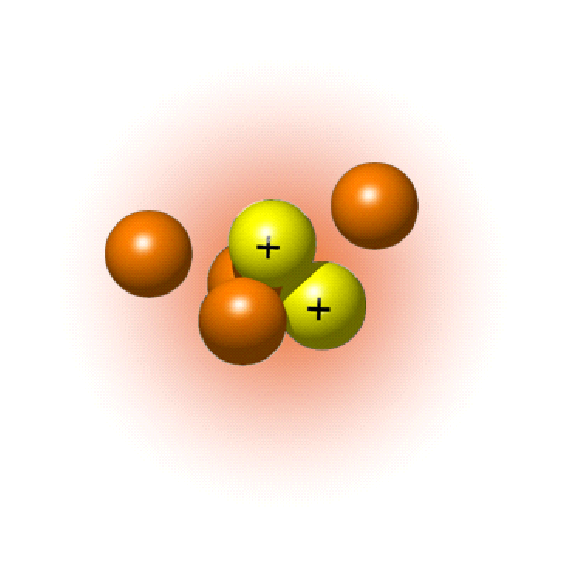
\includegraphics{\images/6He.eps}} \par}
\end{figure}
\column{0.5\linewidth}
\begin{figure}{\par \resizebox*{0.4\textwidth}{!}
{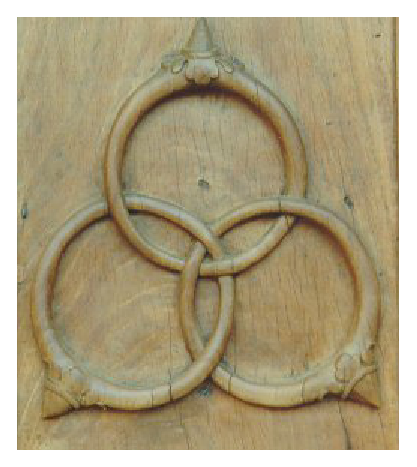
\includegraphics{\images/borromean}} \par}
\end{figure}
\end{columns}
\end{itemize}
\end{frame}





%%%%%%%%%%%%%%%%%%%%%%%%%%%%%%%%%%%%%%%%%%%%%%%%%%%%%%%%
\section{Signatures of weakly-bound nuclei in reaction observables}
%%%%%%%%%%%%%%%%%%%%%%%%%%%%%%%%%%%%%%%%%%%%%%%%%%%%%%%%

\slide{}
\begin{center}
\psframebox[fillcolor=green!10,linecolor=blue,framearc=0.1,fillstyle=solid,framesep=5pt]{
Signatures of weakly-bound nuclei in reaction observables
}%psframe
\end{center} 
\end{frame}

%--------------------------------------
%\slide{Elastic scattering}
%{\bf \brick Let's start from the beginnning $\ldots$ ; Rutherford experiment:}
%\begin{figure}{\par \resizebox*{0.75\textwidth}{!}
%{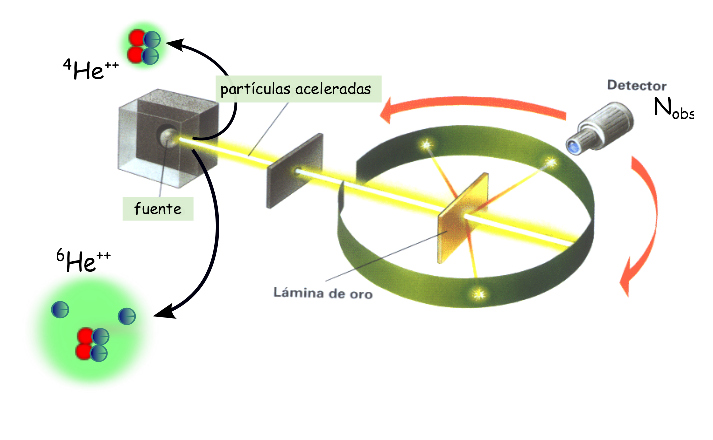
\includegraphics{figs/ruth.eps}} \par}
%\end{figure}
%\end{frame}

%---------------------------------------------
\slide{Elastic scattering: Rutherford experiment...100 years later}
\begin{columns}
\column{0.5\textwidth}
\begin{center}\includegraphics[width=0.8\columnwidth]{figs/he46pb_e19_data.eps}\end{center}
\column{0.5\textwidth}
\begin{center}\includegraphics[width=0.8\columnwidth]{figs/he46pb_e22_data.eps}\end{center}
\end{columns}

\begin{itemize}
\item $^4$He follows Rutherford formula at 19~MeV but not at 22~MeV.
\item $^6$He drastically departs  from Rutherford formula at both energies!
\end{itemize}
\end{frame}


%---------------------------------------------
\slide{Inclusive breakup cross sections}

$$
\psframebox[fillcolor=yellow,linecolor=red,framearc=0.1]{
{\rm ^{6}{He} + ^{208}{Pb} \rightarrow  \alpha + X}
}
$$

\begin{columns}[c]
\column{.5\textwidth}
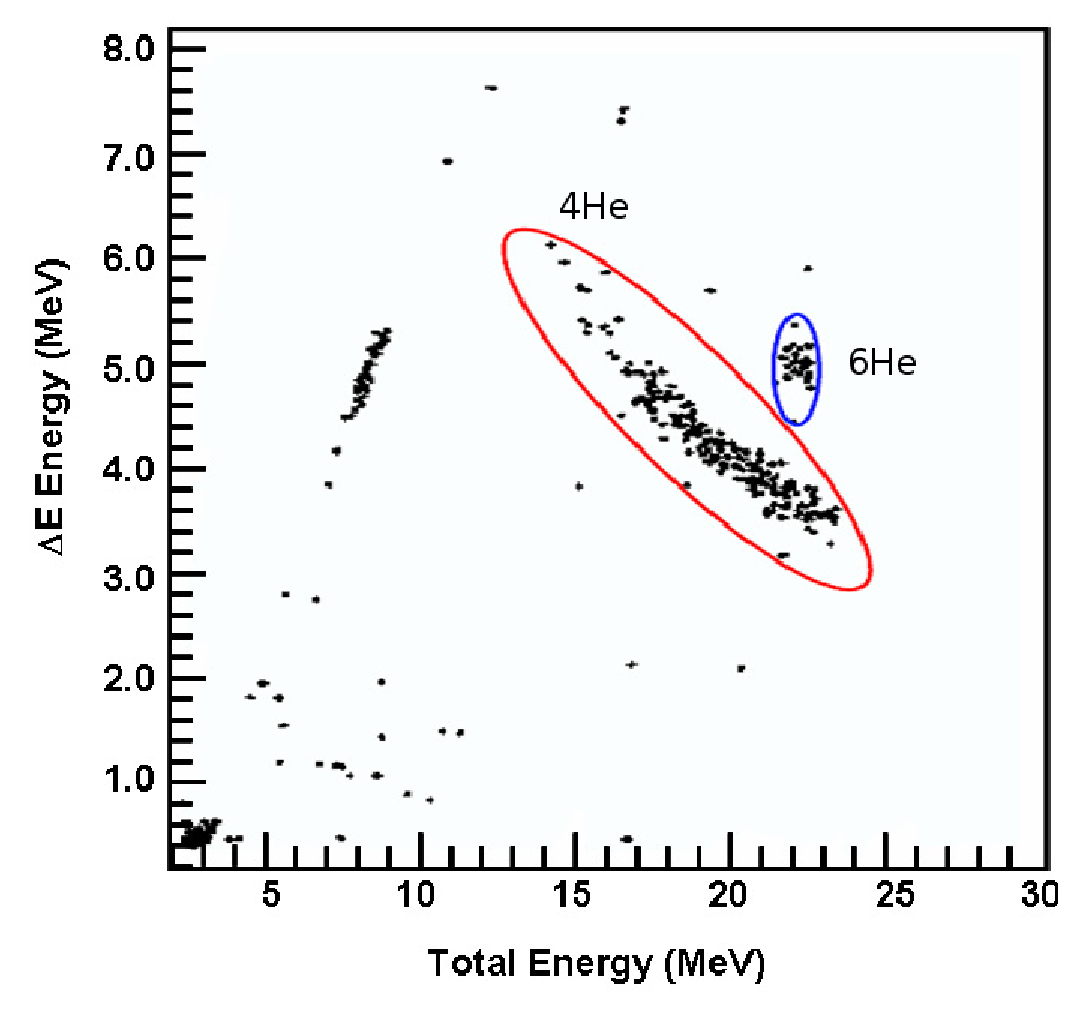
\includegraphics[height=4cm]{\images/bidim-22MeV-new2.eps} 
\column{.5\textwidth}
\includegraphics[height=4cm]{\images/he6pb_e22_pbu_data.eps} 
\end{columns}


%\begin{center}\includegraphics[width=0.55\columnwidth]{\images/he4_he6_ratio_vs_theta.eps}\end{center}

\ding{233}{At large angles, there are more $\alpha$'s than $^{6}$He (elastic) ! } \\
\ding{233}What are the mechanisms behind the $\alpha$ producion and how can we compute it? 

\end{frame}


% --------------------------------------------------------------------------------------
\slide{High-energy interaction cross sections with light targets}

\only<1>{
\ding{32} Interaction cross sections of nuclei on light targets and high energies are proportional to the size of the colliding nuclei.  
%\ding{43} First evidences of the existence of halo nuclei came from reaction cross sections measurements.

\vspace{-0.5cm}

\bc
\column{0.5\linewidth}
$$
\psframebox[fillcolor=yellow,linecolor=red,framearc=0.1]{
\sigma_I \simeq \pi (R_p+R_t)^2
}
$$
\begin{figure}{\par \resizebox*{0.8\textwidth}{!}
{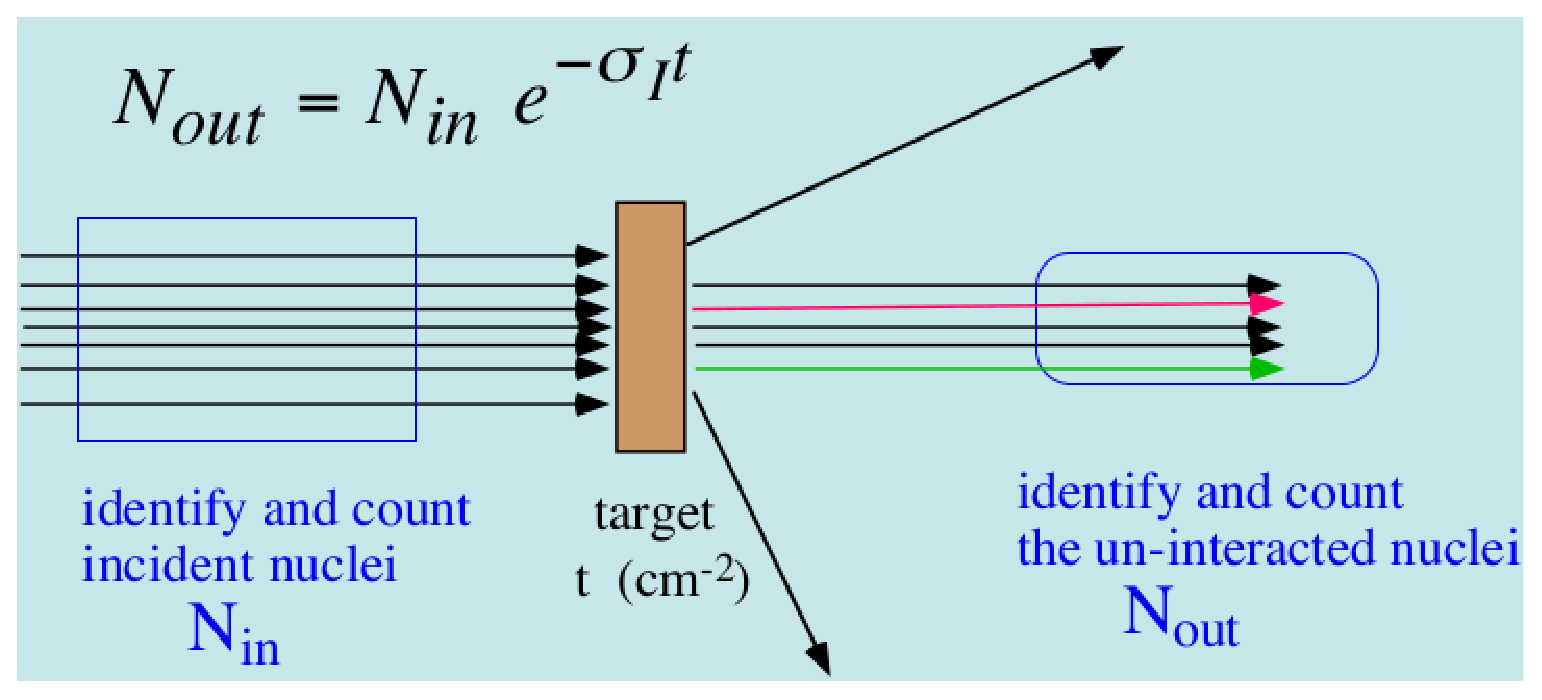
\includegraphics[width=0.95\columnwidth]{\images/interaction_xs.eps}} \par}
\end{figure}
{\small \verde From I.~Tanihata }
\column{0.5\linewidth}
\vspace{0.5cm}
\begin{center}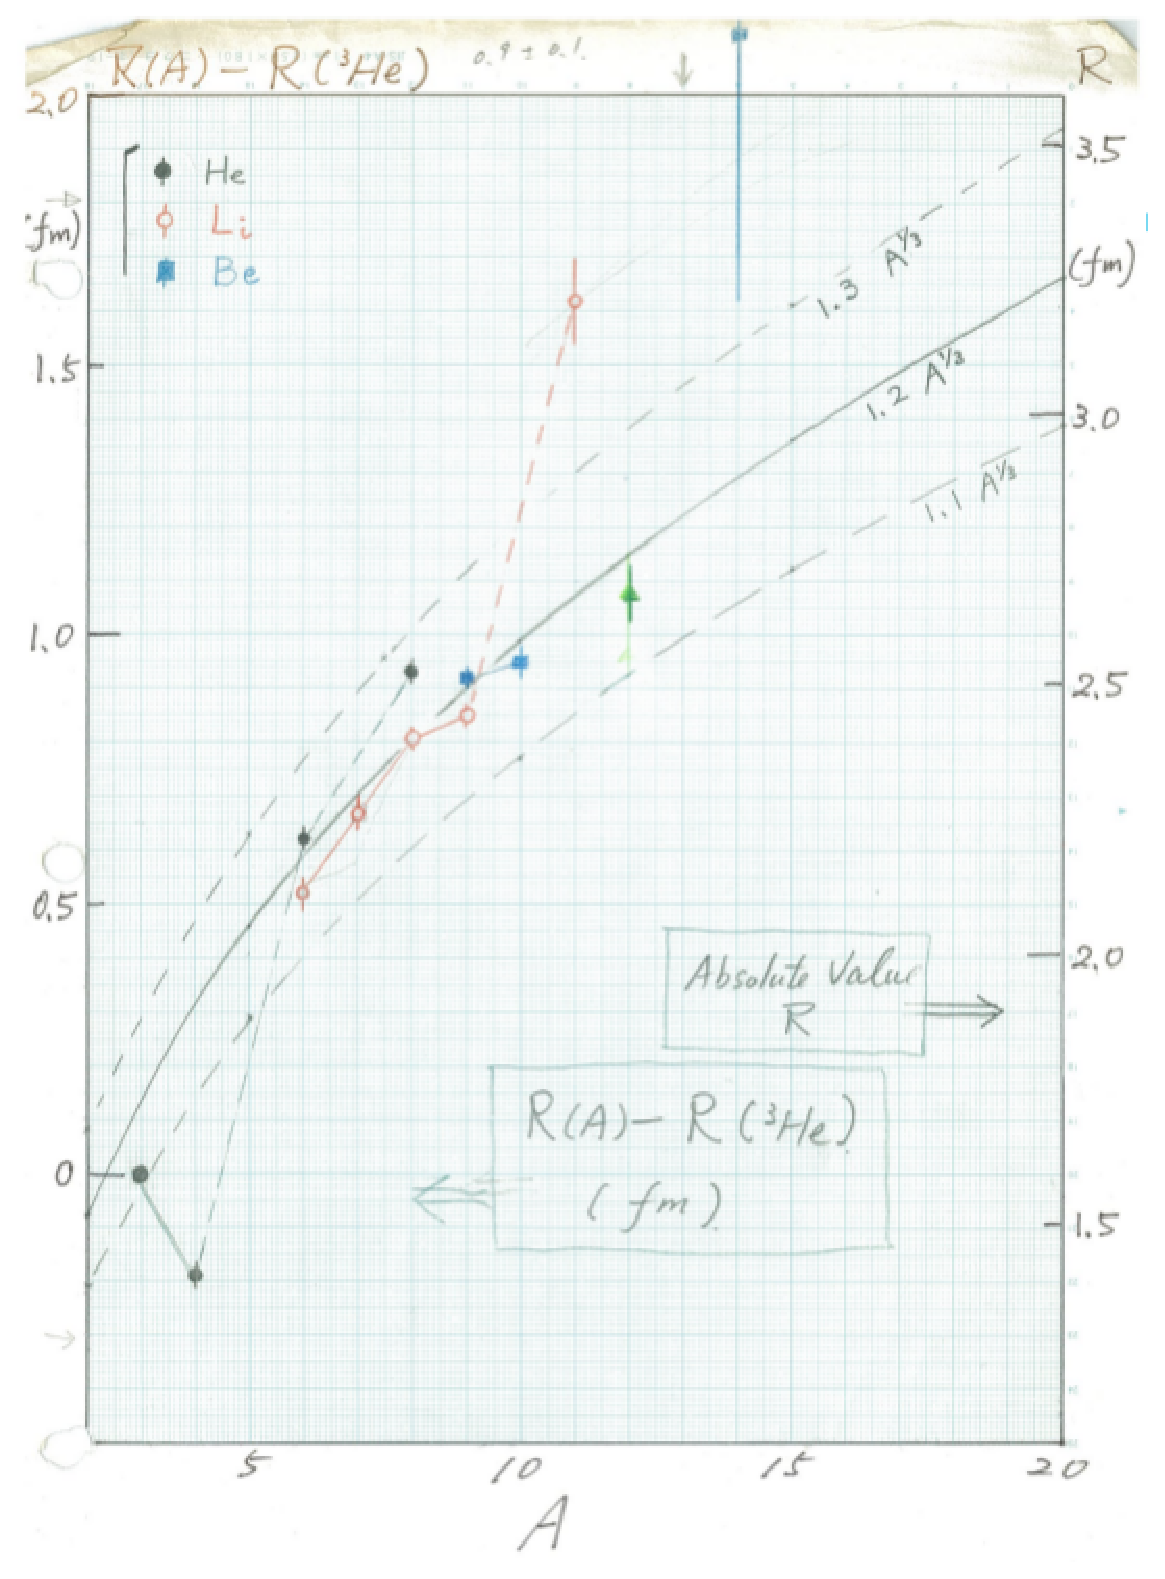
\includegraphics[height=7.0cm]{\images/radios_tanihata_orig.eps}\end{center}
\end{columns}%twocolumn
}%onslide


\only<2>{
\ding{32} Interaction cross sections of nuclei on light targets and high energies (hundreds MeV/nucleon) are proportional to the size of the colliding nuclei.  
%\ding{43} First evidences of the existence of halo nuclei came from reaction cross sections measurements.

\vspace{0.25cm}

\bc
\column{0.6\linewidth}
$$
\psframebox[fillcolor=yellow,linecolor=red,framearc=0.1]{
\sigma_I \simeq \pi (R_p+R_t)^2
}
$$
\begin{figure}{\par \resizebox*{0.5\textwidth}{!}
{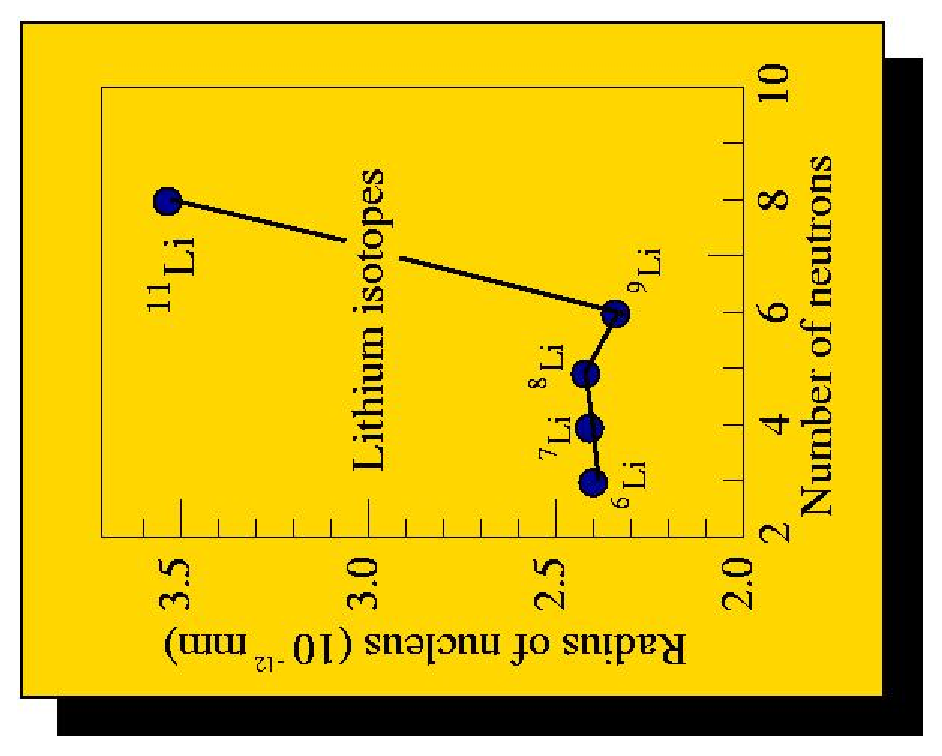
\includegraphics[angle=-90]{\images/liradii.eps}} \par}
\end{figure}
{\small \verde Tanihata {\em et al}, PRL55, 2676 (1985)}
\column{0.4\linewidth}
\vspace{0.5cm}
\begin{center}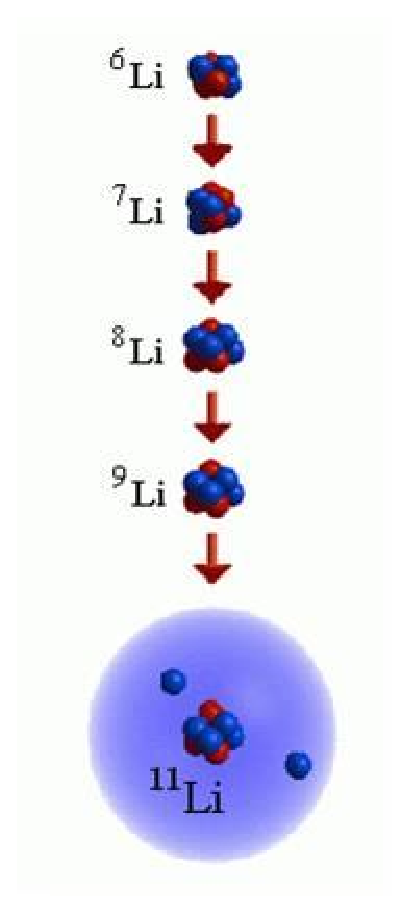
\includegraphics[height=5.0cm]{\images/lithium-isotopes.eps}\end{center}
\end{columns}%twocolumn
}%onslide

\only<3>{
Momentum distributions in breakup reactions
\begin{figure}
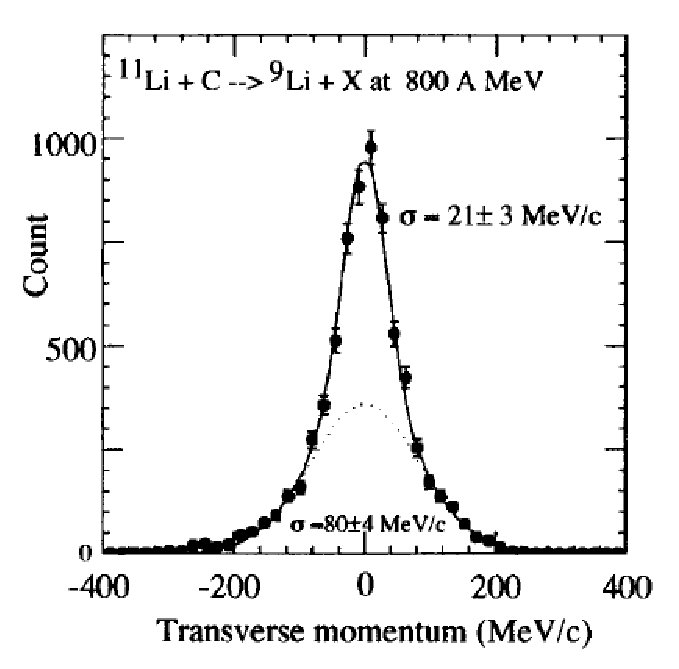
\includegraphics[height=0.6\textheight]{\images/li9momdis.eps}
\end{figure}
\ding{43} {\em \brick A narrow momentum distribution is a signature of  an extended spatial distribuion}
}%onslide

\only<4>{
\begin{figure}
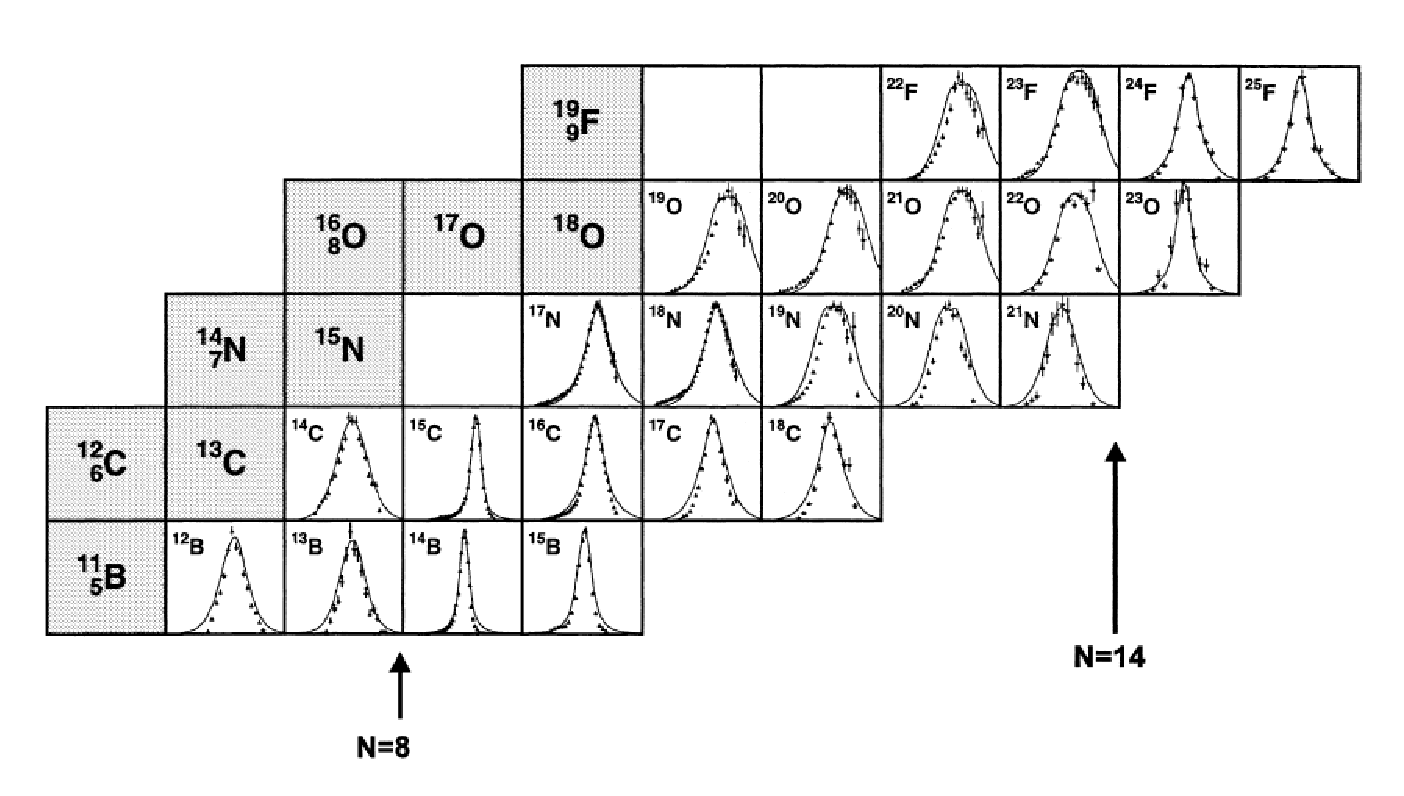
\includegraphics[height=0.7\textheight]{\images/momdis_chart.eps}

\end{figure}
}%only

\end{frame}




\endinput

%----------------------------------
\subsection{Some scattering theory}

\slide{}
\begin{center}
\psframebox[fillcolor=green!10,linecolor=blue,framearc=0.1,fillstyle=solid,framesep=5pt]{
Some scattering theory
}%psframe
\end{center} 
\end{frame}









